\chapter{Design}
\label{ch_design}

This chapter is dedicated to the various modules which comprise the laser tag system being investigated. The system is complex and comprises of many modules both in hardware and software. An overview of the entire system is given followed by the design of the individual modules.

It is important to reiterate at this point the aim of this investigation. This study aims determine the core components of a laser tag module with respect to the tagger and target system. The goal is not to design a ready to play 'user friendly' kit, but rather to determine what modules are required in such a system and how these components perform through the execution of various experiments.

\section{System Overview}

The hardware and software modules of the system will be addressed separately. Figure \ref{fig:system_overview_hardware} gives an overview of the hardware modules required to create a functional laser tag system.

\subsection{Hardware}

\begin{figure}[H]
	\centering
	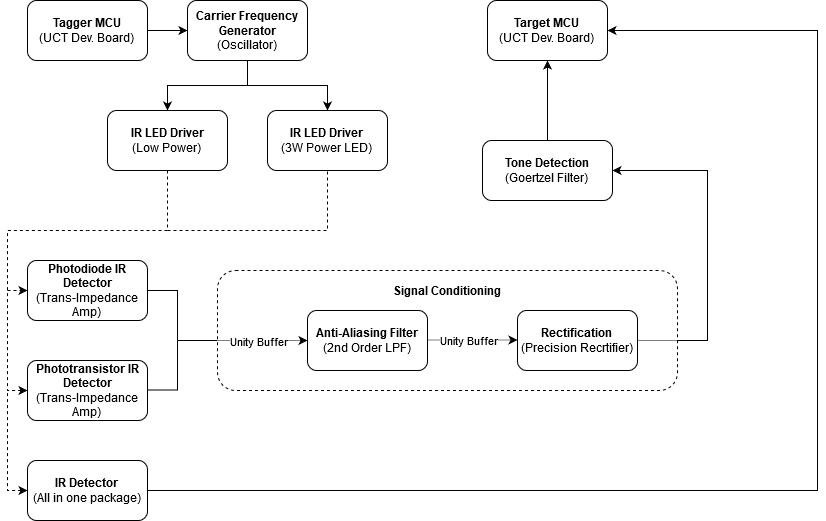
\includegraphics[width=0.9\textwidth]{figures/design/system_overview_hardware}
	\caption{Block Diagram of Hardware Modules}
	\label{fig:system_overview_hardware}
\end{figure}

\subsubsection{Tagger}
The tagger system, in terms of hardware, comprises of a main processor which has been realised on the UCT STM32\footnotemark{} development board. The main processor communicates with the carrier frequency generation module which is responsible for producing the 36kHz square waveform which feeds into the final hardware module of the tagger, the LED driver. Two led driver modules have been design, they both accept the same input signal and are identical in their purpose. The difference between the two modules is in the rated output power, the low power module is designed to drive a typical IR led while the high power module has been designed to drive a high power 3W IR led.

\footnotetext{STM32F051C6}

\subsubsection{Target}
The target system comprises of many more hardware modules, this is due to the comparably higher complexity involved in detecting and processing signals. In addition, to make a comparison between a photodiode and phototransistor possible, a hardware module dedicated to each had to be designed and implemented. The target system hardware consists of three IR sensors, in addition to the two just mentions, an 'all in one' IR receiver device was used to act as a golden measure against which to test the other two receivers.

\section{Hardware Modules}


\section{Software Modules}
